
\begin{figure}
  \begin{subfigure}[t]{0.33\linewidth}
    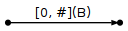
\includegraphics[width=0.8\textwidth]{suffixtree03/suffixtree-1}
    \caption{\#=0}
    \label{suffixtree:fig:1}
  \end{subfigure}
  \begin{subfigure}[t]{0.33\linewidth}
    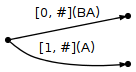
\includegraphics[width=0.8\textwidth]{suffixtree03/suffixtree-2}
        \caption{\#=1}
    \label{suffixtree:fig:2}
  \end{subfigure}
    \begin{subfigure}[t]{0.33\linewidth}
    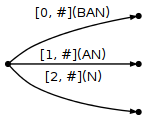
\includegraphics[width=0.8\textwidth]{suffixtree03/suffixtree-3}
        \caption{\#=2}
    \label{suffixtree:fig:3}
  \end{subfigure}
  \begin{subfigure}[t]{0.33\linewidth}
    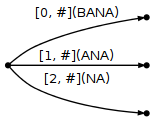
\includegraphics[width=0.8\textwidth]{suffixtree03/suffixtree-4}
    \caption{\#=3}
    \label{suffixtree:fig:4}
  \end{subfigure}
  \begin{subfigure}[t]{0.33\linewidth}
    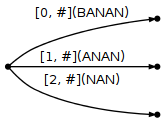
\includegraphics[width=0.8\textwidth]{suffixtree03/suffixtree-5}
        \caption{\#=4}
    \label{suffixtree:fig:5}
  \end{subfigure}
    \begin{subfigure}[t]{0.33\linewidth}
    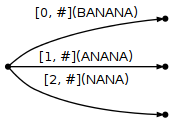
\includegraphics[width=0.8\textwidth]{suffixtree03/suffixtree-6}
        \caption{\#=5}
    \label{suffixtree:fig:6}
  \end{subfigure}
  \caption{前六轮迭代(\#从0到5)中的后缀树变化}
  \label{suffixtree:fig:0to5}
\end{figure}
\begin{figure}
  \begin{subfigure}[t]{0.5\linewidth}
    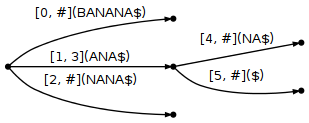
\includegraphics[width=\textwidth]{suffixtree03/suffixtree-7-1}
    \caption{remainder=4}
    \label{suffixtree:fig:7-1}
  \end{subfigure}
  \begin{subfigure}[t]{0.5\linewidth}
    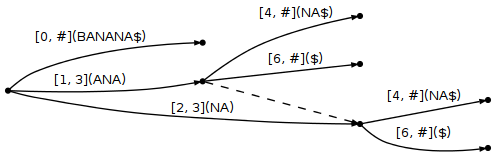
\includegraphics[width=\textwidth]{suffixtree03/suffixtree-7-2}
        \caption{remainder=3}
    \label{suffixtree:fig:7-2}
  \end{subfigure}
  \begin{subfigure}[t]{0.5\textwidth}
    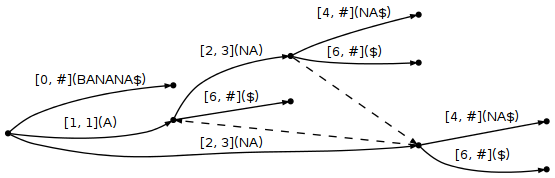
\includegraphics[width=\textwidth]{suffixtree03/suffixtree-7-3}
    \caption{remainder=2}
    \label{suffixtree:fig:7-3}
  \end{subfigure}
  \begin{subfigure}[t]{0.5\textwidth}
    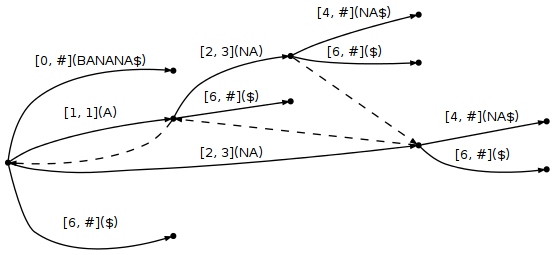
\includegraphics[width=\textwidth]{suffixtree03/suffixtree-7-4}
    \caption{remainder=1}
    \label{suffixtree:fig:7-4}
\end{subfigure}
\caption{最后一轮迭代(\#=6)时的后缀树}
\label{suffixtree:fig:7}
\end{figure}

%%% Local Variables: 
%%% mode: latex
%%% TeX-master: "../main"
%%% End: 
